\documentclass[11pt,a4paper,twoside]{article}
\usepackage[utf8]{inputenc}
\usepackage{polski}



\usepackage{graphicx}
\usepackage{subcaption} % obrazki obok siebie
%\usepackage[caption=false]{subfig} % obrazki nad sobą
\usepackage{wrapfig} 
\usepackage{float}
\usepackage{geometry}
%\geometry{lmargin=3cm,rmargin=2cm, tmargin=2.5cm, bmargin=2.5cm} %marginesy w pracy inż/mgr
\geometry{lmargin=2.5cm,rmargin=2.5cm, tmargin=2.5cm, bmargin=2.5cm} %marginesy ogólne
\usepackage{multirow} % scalanie wierszy tabeli

\usepackage{fancyhdr}
\pagestyle{fancy}
\fancyhead{} % wszystkie nagłówki puste
%\fancyhead[RE,LO]{ Absolwenci Wydziału Prawa  2012}
\fancyfoot{} % wszystkie stopki puste
\fancyfoot[LE,RO]{\thepage}
\renewcommand{\headrulewidth}{0pt}
%\renewcommand{\footrulewidth}{0.4pt}

\usepackage{hyperref}% nazwy odsyłaczy

%unikanie myślników dzielących słowa między liniami
\tolerance=1
\emergencystretch=\maxdimen
\hyphenpenalty=10000
\hbadness=10000

\usepackage{algorithm}
\usepackage{algorithmicx}
\usepackage{algpseudocode}
\makeatletter
\renewcommand{\ALG@name}{Algorytm}
\renewcommand{\figurename}{Wykres}

\usepackage{enumitem}
\setitemize{itemsep=2pt,topsep=2pt,parsep=2pt,partopsep=2pt} %odstępy wyliczanych elementów (-)

\usepackage{indentfirst} % wcięcie w pierwszym akapicie (pod)rozdziału
%%%%%%%%%%%%%%%%%%%%%%%%%%%%%%%%%%%%%%%%% formatowanie kodu R
\usepackage{listings} 
\usepackage{color}
\definecolor{gray}{rgb}{0.5,0.5,0.5}
\lstset{
language=R,
basicstyle=\footnotesize\ttfamily,%\scriptsize\ttfamily,
commentstyle=\ttfamily\color{gray},
numbers=left,
numberstyle=\ttfamily\color{gray}\footnotesize,
stepnumber=0, % numeracja linii
numbersep=5pt,
backgroundcolor=\color{white},
showspaces=false,
showstringspaces=false,
showtabs=false,
frame=none, % obramowanie kodu
tabsize=2,
captionpos=b,
breaklines=true,
breakatwhitespace=false,
title=\lstname,
escapeinside={},
keywordstyle={},
morekeywords={}
}
%%%%%%%%%%%%%%%%%%%%%%%%%%%%%%%%%%%%%%%%%

%%% zawijanie tekstu w tabelach zgodnie z życzeniem
\usepackage{stackengine}
\usepackage{array}
\newcolumntype{L}[1]{>{\raggedright\arraybackslash}p{#1}}
\setstackEOL{\#}
\setstackgap{L}{12pt}
%%%

\usepackage{amsfonts} % zbiory liczba (np. naturalnych)
\usepackage{amsmath} %duże klamry
\usepackage{bbm} %skok jednostkowy
\usepackage[titletoc,title]{appendix} % dodatki - zmiana wyświetlania nagłówka
\pagenumbering{gobble}
\usepackage{afterpage} % pusta strona
\usepackage{tabularx}

\usepackage{makecell}

%\usepackage{setspace} % interlinia
%\singlespacing 
%\onehalfspacing
%\doublespacing
%\setstretch{0.96}

\begin{document}

\begin{center}
\vspace*{3\baselineskip}
{\LARGE{PORR Projekt}}
\\
\vspace*{1\baselineskip}
{\large{Algorytm świetlika (FA) i roju świetlików (GSO) do rozwiązania problemu plecakowego.}}
\\
\vspace*{1\baselineskip}
Cezary Dubiel, 251387\\
Tomasz Korzeniowski, 265753\\
\vspace*{1\baselineskip}
\today
\end{center}
\section{Zadanie}
Zdefiniować i rozwiązać dwa zadania o różnej złożoności. Zrealizować zadania w wersji sekwencyjnej i równoległej. Opisać przyśpieszenie obliczeń w zależności od stopnia zrównoleglenia (porównać obie metody - FA i GSO). Przedstawić graficznie zbieżność obu algorytmów w wersji sekwencyjnej - wartości funkcji celu w kolejnych iteracjach.
\section{Podstawy teoretyczne}
\subsection{Problem plecakowy}
Problem plecakowy polega na zapakowaniu maksymalnie cennego zbioru przedmiotów do plecaka, tak by nie przekroczyć jego ładowności. Można wyróżnić dwa podejścia do liczby pakowanych przedmiotów. W ogólnym podejściu zakładamy, że posiadamy wiele ($1, 2, \ldots$) egzemplarzy każdego z $N$ różnych przedmiotów. W bardziej rzeczywistych przypadkach posiadamy dokładnie jeden egzemplarz każdego z $N$ różnych przedmiotów. W tym projekcie zajmiemy się drugim podejściem.

Zakładamy, że mamy do dyspozycji $n \in N$ przedmiotów. Każdy z tych przedmiotów jest warty $c$, a także posiada swoją wagę $m$. Naszym zadaniem jest zdecydowanie czy i które z przedmiotów załadujemy, tak by ich sumaryczna masa nie przekroczyła ładowności plecaka $M_{max}$. Model matematyczny problemu plecakowego można przedstawić następująco
\begin{equation}
\max \sum_{i}^{N} c_{i} x_{i} 
\label{f_celu}
\end{equation}
\begin{equation}
\sum_{i}^{N} m_{i} x_{i} \leq M_{max}
\end{equation}
\begin{equation}
x_{i} \in \{0,1\}
\end{equation}

Zatem poszukujemy rozwiązania w postaci binarnego wektora $x$ długości $N$:
$$x_{i} = 
	\begin{cases} 
      1, & \text{gdy i-ty przedmiot zostanie zapakowany do plecaka} \\
      0, & \text{w przeciwnym przypadku}\\
   \end{cases}
$$

Jeśli przyjmiemy, że posiadamy sześć przedmiotów, które możemy spakować, a także znamy $C = [c_{i}]_{1\times N}$, $M = [m_{i}]_{1\times N}$ oraz wektor $x = (0, 1, 0, 0, 1, 1)$ to wiemy, że do plecaka został załadowany przedmiot drugi, piąty oraz szósty. 

\subsection{Algorytm świetlika}
Algorytm świetlika (FA - ang. \textit{firefly algorithm}) jest heurystyką inspirowaną zachowaniem społecznym świetlików (robaczków świętojańskich). Jego głównym zastosowaniem są zadania optymalizacji ciągłej z ograniczeniami. Może jednak być wykorzystywany także w problemach optymalizacji kombinatorycznej.

Fenomen świetlików polega na ich bioluminescencyjnej komunikacji. Każdy z nich cechuje się pewną atrakcyjnością, proporcjonalną do jasności z jaką świecą. Świetlik o większej jasności przyciąga inne osobniki (przyjmujemy obupłciowość świetlików) o mniejszej jasności. Zakładamy też, że świetliki nie umierają.

Na początku działania algorytmu losowana jest populacja świetlików. Każdy z nich reprezentuje pewne rozwiązanie problemu, czyli poszukiwany wektor $x$. Jego jasnością jest wartość funkcji celu dla danego rozwiązania. Następnie poszukiwany jest najlepszy ze świetlików (pod względem jasności - wartości funkcji celu), a pozostałe poruszają się w jego kierunku. Ruch $i$-tego świetlika zależy od wartości funkcji atrakcyjności $\beta_{i}$
\begin{equation}
\beta_{i} = \beta_{0} e^{-\gamma r_{ij}^{2}}
\end{equation}
gdzie $\beta_{0}$ (maksymalna atrakcyjność) oraz $\gamma$ (współczynnik absorpcji) są ustalonymi na wstępie parametrami algorytmu, a $r_{ij}^{2}$ to odległość między świetlikami $i$ oraz $j$.

Ruch świetlika $i$ przyciąganego do bardziej atrakcyjnego świetlika $j$ jest następujący
\begin{equation}
x_{i} = x_{i} + \beta_{i}(x_{j} - x_{i}) + u_{i} 
\label{moveFA}
\end{equation}
gdzie $u_{i}$ jest wektorem liczb losowych wygenerowanych z rozkładem równomiernym z przedziału [0,1]. Jeśli świetlik nie znajdzie się w sąsiedztwie innego świetlika o większej jasności wówczas wykonywane jest jego losowe przesunięcie $u_{i}$.

Algorytm świetlika można przedstawić w postaci pseudokodu
%\begin{algorithm}[ht]
%\caption{Algorytm świetlika (FA)}
%\label{FA}
%\begin{algorithmic}%[1]
%\Require $C$, $M$, $\beta_{i}$, $\gamma$
%	\State wylosuj populację świetlików
%	\For {iter=1 to MAX-ITER}
%	\State oblicz wartość funkcji celu (\ref{f_celu}) dla każdego świetlika
%	\State znajdź najlepszego świetlika
%	\State przemieść pozostałe świetliki w stronę znalezionego najlepszego zgodnie z (\ref{moveFA})
%	\EndFor		
%\end{algorithmic}
%\end{algorithm}

\begin{algorithm}[ht]
\caption{Algorytm świetlika (FA)}
\label{FA}
\begin{algorithmic}%[1]
\Require $C$, $M$, $k$, $\beta_{i}$, $\gamma$
	\State wylosuj populację świetlików
	\While{ nie osiągnięto warunku stopu}
	\For {i=1 to k}
		\For{j=1 to k}
			\If{$f(x_{j}) > f(x_{i})$}
				\State oblicz odległość $r_{ij}$
				\State zmodyfikuj atrakcyjność $\beta_{i}$
				\State wygeneruj losowy wektor $u_{i}$
				\State utwórz nowe rozwiązanie zgodnie z (\ref{moveFA})
    		\EndIf
		\EndFor
	\EndFor	
	\State wygeneruj losowy wektor $u_{b}$
	\State przesuń najlepszego świetlika $x_{b} = x_{b} + u_{b}$
	\EndWhile	
\end{algorithmic}
\end{algorithm}

$f(x_{j})$ oznacza wartość funkcji celu dla świetlika $x_{j}$. Warunkiem stopu algorytmu może być zadana liczba iteracji. Do sprawdzenia zbieżności algorytmu warunkiem stopu będzie brak zmian rozwiązania (na pewnym poziomie) przed zadaną liczbę iteracji.

\clearpage
\subsection{Algorytm roju świetlików}
Algorytm roju świetlików (GSO - ang. \textit{glowworm swarm optimization}), w przeciwieństwie do FA, oparty jest na zachowaniach społecznych nieskrzydlatych świetlików. Przejawia się to zdolnością do zmiany intensywności emisji lucyferny, czyli wydawaniem blasków o różnym natężeniu. Od algorytmu świetlika, GSO różni się także ze względu na możliwość podziału świetlików na podgrupy. Pozwala to osiągać wiele lub nawet wszystkie optima lokalne.

Różna jest także reprezentacja sąsiedztwa świetlików. Zmienna sąsiedztwa $r_{d}$ jest związana z zakresem radialnym $r_{s}$, tak aby $0 < r_{d} \leq r_{s}$. Wynika z tego, że świetlik $i$ bierze pod uwagę świetlika $j$ jako sąsiada, jeśli $j$ jest wewnątrz obszaru sąsiedztwa rozwiązania $i$ oraz poziom lucyferny jest wyższy dla $j$-tego niż $i$-tego.

Algorytm rozpoczyna się od losowego rozmieszczenia świetlików, a także przypisaniu im wielkość lucyferny równą 0. Przebieg algorytmu składa się z 3 faz głównych. W fazie pierwszej następuje modyfikacja poziomu lucyferny, czyli wyznaczenie wartości funkcji celu. W oryginalnej wersji algorytmu odejmuje się część lucyferny w celu symulacji mechanizmu rozkładu tej substancji w czasie. Ze względu na to, że przedmioty przynoszą stały zysk wynikający z ich zapakowania, zrezygnujemy z takiego pomniejszania.

Kolejnym krokiem jest faza ruchu. Wyznaczane jest prawdopodobieństwo przemieszczenia świetlika $i$ w kierunku $j$ w chwili $t$ zgodnie ze wzorem
\begin{equation}
p_{ij}(t) = \frac{l_{j}(t)-l_{i}(t)}{\sum_{k\in N_{i}(t)} l_{k}(t) - l_{i}(t)}
\label{p-stwoPrzemieszczenia}
\end{equation}
\begin{equation}
N_{i}(t) = \{j: d_{ij}(t) < r_{d}(t) ; l_{i}(t) < l_{j}(t)\}
\label{zbiorSasiadow}
\end{equation}
gdzie $N_{i}(t)$ to zbiór sąsiadów świetlika $i$, a $d_{ij}(t)$ odległość między świetlikiem $i$ oraz $j$.

Następnie świetliki są przemieszczane zgodnie z 
\begin{equation}
x_{i}(t+1) = x_{i}(t) + s\frac{x_{j}(t) - x_{i}(t)}{\Vert x_{j}(t) - x_{i}(t) \Vert}
\label{przemieszczenie}
\end{equation}
gdzie $s > 0$ oznacza rozmiar kroku przemieszczenia.

Ostatnią fazą jest modyfikacja zakresu sąsiedztwa.
\begin{equation}
r_{d}(t+1) = \min \bigg\{ r_{s}, \max \big\{0, r_{d}(t)+\beta(n_{t} - |N_{i}(t)|) \big\} \bigg\}
\label{zakresSasiedztwa}
\end{equation}
gdzie $\beta$ to pewna stała, a $n_{t}$ jest parametrem używanym do sterowania liczbą świetlików w sąsiedztwie.

\begin{algorithm}[ht]
\caption{Algorytm roju świetlików (GSO)}
\label{GSO}
\begin{algorithmic}%[1]
\Require $C$, $M$
	\State wylosuj populację świetlików
	\While{ nie osiągnięto warunku stopu}
	\State zmodyfikuj poziom lucyferny każdego świetlika
	\State przemieść każdego świetlika (\ref{zbiorSasiadow})
	\For {każdego świetlika $j \in N_{i}(t)$}
		\State wyznacz prawdopodobieństwo przemieszczenia (\ref{p-stwoPrzemieszczenia})
		\State przemieść świetliki (\ref{przemieszczenie})
		\State zmodyfikuj zakres sąsiedztwa (\ref{zakresSasiedztwa})
	\EndFor	
	\EndWhile	
\end{algorithmic}
\end{algorithm}

\section{Wybrane technologie}
Implementacja algorytmów została wykonana w języku C++ 11. Do implementacji i testów wykorzystano zintegrowane środowisko programistyczne Code Blocks .

Do realizacji wersji równoległej algorytmów z pamięcią wspólną wykorzystano środowisko OpenMP.

\subsection{Sprzęt}
\bgroup
\def\arraystretch{1.3}
\begin{tabular}{rl}
\centering
%\begin{tabularx}{\textwidth}{lX}
%\hline
 Procesor & Intel Core i7-4770K 3.5 GHz, 4 rdzenie, 8 wątków  \\
 & (korzystanie z hiper-wątków)\\
 Pamięć RAM &  16 GB\\
 System operacyjny & Windows 7 \\ 

\end{tabular}
\egroup

\section{Wyniki}
Dla każdego z algorytmów wykonano 10 symulacji rozwiązania problemów o różnych złożonościach (liczbie możliwych elementów do spakowania). Symulacje te zostały wykonane w wersji sekwencyjnej oraz równoległej dla czterech i ośmiu wątków. Większej liczby wątków nie ma sensu rozważać, ponieważ używany sprzęt nie wystarczy do większego zrównoleglenia obliczeń.
\subsection{Przyśpieszenie obliczeń}
Obliczenia były prowadzone przy założeniach, że rozpatrujemy populację dwustu świetlików, a maksymalna liczba iteracji jaką może wykonać algorytm to tysiąc. Zestawienie czasów wykonania programu i osiągniętego przyśpieszenia w zależności od zrównoleglenia prezentują tabele \ref{wspólnaFA} i \ref{wspólnaGSO}.

\bgroup
\def\arraystretch{1.1}
\begin{table}[ht]
\caption{Czas i przyśpieszenie wykonania algorytmu świetlika (FA)}
\label{wspólnaFA}
\centering
\begin{tabular}{|c||c||c|c||c|c|}
\hline
 \multirow{2}{*}{złożoność} & \multirow{2}{*}{sekwencyjnie} & \multicolumn{2}{c||}{4 wątki} & \multicolumn{2}{c|}{8 wątków} \\\cline{3-6}
 & & czas & przyśpieszenie & czas & przyśpieszenie \\\hline
 24  & 0,0753906 & 0,17625 & 0,42775 &  0,0847009 & 0,89008\\\hline
 120  & 0,215828 & 0,46174 & 0,46742 & 0,302861 & 0,71263 \\\hline
 600  & 1,27815 & 1,23022 & 1,03896 & 0,747475 & 1,70996 \\\hline
 960  & 1,51908 & 1,1197 & 1,35668 & 0,698841 & 2,17371 \\\hline
\end{tabular}
\end{table}
\egroup

\bgroup
\def\arraystretch{1.1}
\begin{table}[ht]
\caption{Czas i przyśpieszenie wykonania algorytmu roju świetlików (GSO)}
\label{wspólnaGSO}
\centering
\begin{tabular}{|c||c||c|c||c|c|}
\hline
 \multirow{2}{*}{złożoność} & \multirow{2}{*}{sekwencyjnie} & \multicolumn{2}{c||}{4 wątki} & \multicolumn{2}{c|}{8 wątków} \\\cline{3-6}
 & & czas & przyśpieszenie & czas & przyśpieszenie \\\hline
 24  & 0,0963501 & 0,3246547 & 0,29678 &  0,3521662 & 0,27359\\\hline
 120  & 0,245403 & 0,237385 & 0,91779 & 0,214741 & 1,14279 \\\hline
 600  & 0,813467 & 0,612114 & 1,32895 & 0,661251 & 1,23019 \\\hline
 960  & 1,30946 & 0,892147 & 1,46776 & 0,711577 & 1,84022 \\\hline
\end{tabular}
\end{table}
\egroup
\vspace*{1\baselineskip}

\subsection{Zbieżność algorytmów}
\begin{figure}[ht]
%\vspace{-20pt}
\centering
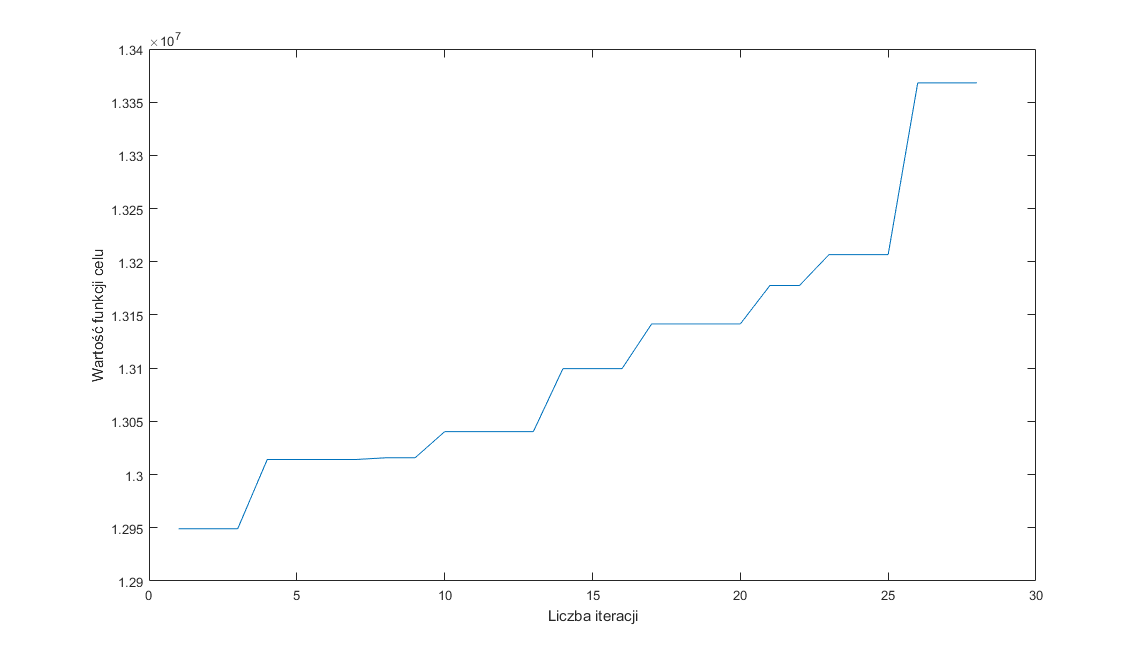
\includegraphics[height=8.4cm, width=15.7cm]{zbieznoscFA24}
\caption{Zbieżność algorytmu świetlika (FA) dla 24 elementów.}
\label{zbieznoscFA24}
\end{figure}

\begin{figure}[ht]
%\vspace{-20pt}
\centering
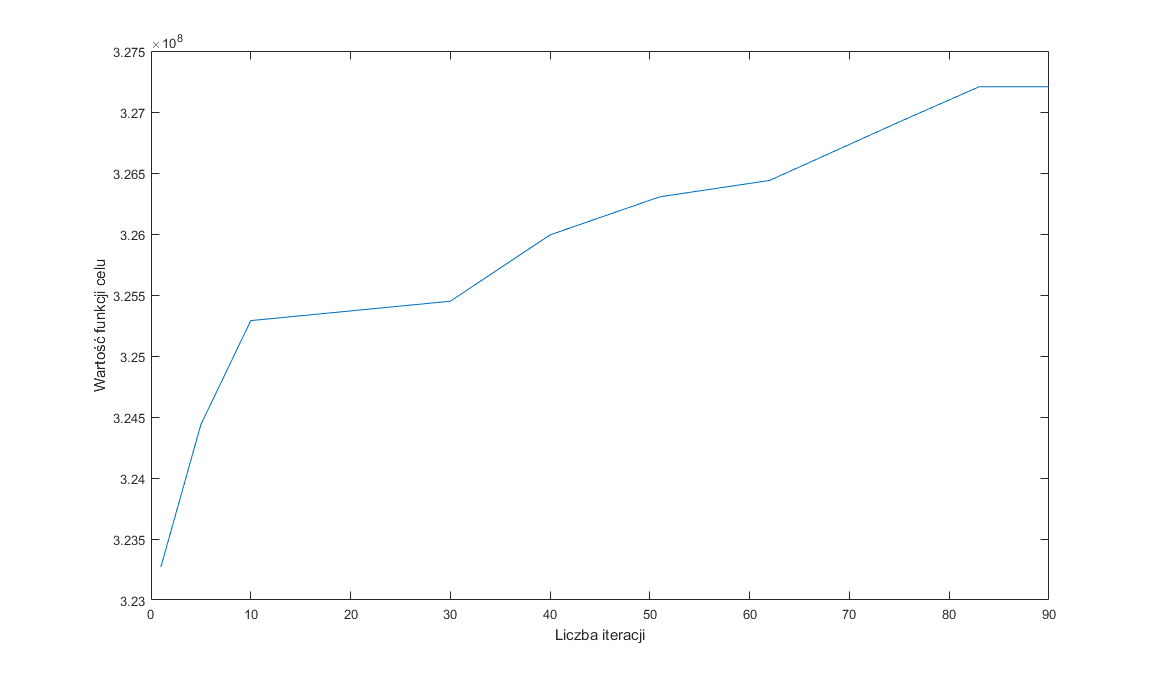
\includegraphics[height=8.4cm, width=15.7cm]{zbieznoscFA600}
\caption{Zbieżność algorytmu świetlika (FA) dla 600 elementów.}
\label{zbieznoscFA600}
\end{figure}
%\clearpage

W każdym z testów znane było najlepsze rozwiązanie  problemu plecakowego na podstawie którego wyznaczony był $\epsilon$. Jest to parametr wykorzystywany do wyznaczania zbieżności oznaczający procentową wartość o jaką może różnić się rozwiązanie znalezione przez algorytm w stosunku do rozwiązania optymalnego. Na potrzeby testów został on ustalony $\epsilon = 0.04$. Przez zbieżność algorytmu rozumiemy dostatecznie bliskie rozwiązanie w stosunku do rozwiązania optymalnego, które nie zmienia się przez określoną liczbę iteracji.

Na podstawie wykresów \ref{zbieznoscFA24} i \ref{zbieznoscFA600} można zauważyć, że liczba iteracji potrzebnych do rozwiązania problemu na założonym poziomie dokładności rośnie wraz z rozmiarem problemu. Ponadto dla problemów o dużych rozmiarach (600 elementów) charakterystyczny jest większy początkowy wzrost wartości funkcji celu w stosunku do dalszych iteracji.

Algorytm roju świetlików (GSO) nie nadaje się naszym zdaniem do problemów dyskretnych. Początkowo wylosowane najlepsze rozwiązanie pozostaje nim aż do końca działania algorytmu. Świetliki poruszają się wokół lokalnych maksimów, lecz liderzy (najlepsze lokalne rozwiązania) mają zbyt małe możliwości poruszania się.


%\newpage

%\clearpage
%\newpage
\begin{thebibliography}{9}
%\addcontentsline{toc}{section}{Literatura}
%\bibitem{BOCD}
%Z. Michalewicz, D. B. Fogel
%\emph{Jak to rozwiązać czyli nowoczesna heurystyka}.
%WNT, Warszawa 2006
\bibitem{knapsack}
\url{http://www-users.mat.uni.torun.pl/~henkej/knapsack.pdf}
\bibitem{knapsack2}
\url{http://pe.org.pl/articles/2014/6/37.pdf}
\bibitem{knapsack3}
\url{http://home.agh.edu.pl/~slukasik/pub/021_Lukasik_KAEiOG2011(presentation).pdf}
\bibitem{knapsack4}
\url{https://eti.pg.edu.pl/documents/176546/25263566/SZ_wyklad2.pdf}

\end{thebibliography}
\end{document}
